\chapter{基于BLE Mesh的智能家居平台实现}
\section{开发语言的选择}
现今,市面上有许多开发语言可供选择,它们各自有各自的优点,如C/C++语言执行速度快,程序占用空间小;Go语言代码简洁,执行速度快;Dart语言易于编写,使用Flutter框架后还可实现一套代码就能编译出iOS/Android端的App。

对于本项目的BLE Mesh节点而言,其性能不高且存储空间狭小,并且需使用Nordic芯片厂商所提供的nRF5 SDK for Mesh,因此选择了C语言作为开发语言。

对于本项目的网关端而言,其性能充足但需要高扩展性且逻辑复杂,为了开发方便,因此选择了Go语言作为开发语言。

对于本项目的移动端而言,需要同时支持Android与iOS系统,为了界面逻辑统一,因此选择了Dart语言与Flutter框架作为开发语言。

\section{集成开发环境的选择}
在BLE Mesh节点开发上,目前针对嵌入式开发并支持C语言主要是SEGGER Embedded Studio及Keil,SEGGER Embedded Studio相较于Keil更加易用,并且能很好地兼容nRF5 SDK for Mesh,因此选择了SEGGER Embedded Studio作为BLE Mesh节点的集成开发环境。

在网关端开发上,目前针对Go语言的集成开发环境主要有GoLand与VS Code,但GoLand功能更为强大,能很好地进行调试以及包管理,因此选择了GoLand作为网关端的集成开发环境。

在移动端开发上,目前Google推荐使用Android Studio进行Dart+Flutter的开发,因此选择了Android Studio作为移动端的集成开发环境。

\section{逻辑部分的实现}
\subsection{BLE Mesh节点}
BLE Mesh节点主要分为两个角色,一个是Server,一个是Provisioner。Server作为连接继电器、传感器等模块的角色,而Provisioner则负责给未配置的Server节点发放BLE Mesh网络配置。本项目采用Nordic的nRF5 SDK for Mesh来处理BLE Mesh协议栈的底层调用。

\subsubsection{Server}
Server节点在上电后初始化BLE、Mesh协议栈及其他参数,开始发送Unprovisioned Node Beacon广播信息,等待Provisioner分发配置,配网成功后注册GATT服务与传感器服务,以便移动端或网关端BLE Mesh插件通过此节点代理入网,并允许其他节点访问它的模块。

\begin{figure}[H]
    \centering
    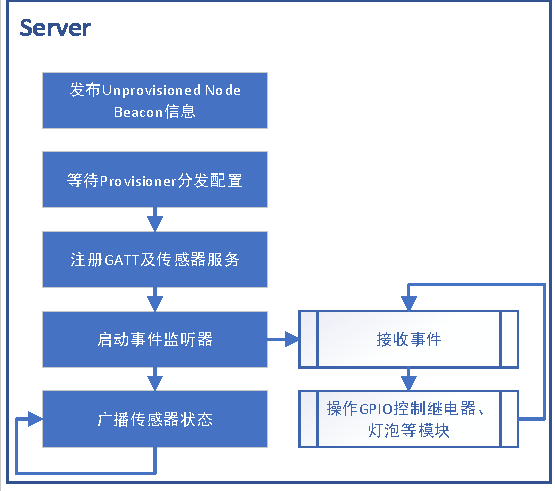
\includegraphics{flowchart_mesh_server.pdf}
    \caption{基于BLE Mesh的智能家居平台BLE Mesh Server节点流程图}
    \label{fig:flowchart_mesh_server}
\end{figure}

\begin{figure}[H]
    \centering
    \begin{lstlisting}[language=C]
    ble_stack_init();
    gap_params_init();
    conn_params_init();
    mesh_init();
    //初始化蓝牙协议栈、GATT参数、传感器参数、Mesh协议栈
    if (!m_device_provisioned){
        //设备未配网
        static const uint8_t static_auth_data[NRF_MESH_KEY_SIZE] = STATIC_AUTH_DATA;
        //配置OOB预认证密钥
        mesh_provisionee_start_params_t prov_start_params = {
            .p_static_data    = static_auth_data,
            .prov_complete_cb = provisioning_complete_cb,
            .prov_device_identification_start_cb = device_identification_start_cb,
            .prov_device_identification_stop_cb = NULL,
            .prov_abort_cb = provisioning_aborted_cb,
            .p_device_uri = EX_URI_LS_SERVER
        };
        mesh_provisionee_prov_start(&prov_start_params);
        //启动Provisionee过程,等待配网结束
    }
    mesh_app_uuid_print(nrf_mesh_configure_device_uuid_get());
    //输出配网后分配到的设备UUID以供调试使用
    mesh_stack_start();
    //启动Mesh协议栈
    \end{lstlisting}
    \caption{基于BLE Mesh的智能家居平台BLE Mesh Server节点关键代码}
    \label{fig:code_mesh_server}
\end{figure}

\subsubsection{Provisioner}
Provisioner节点上电后初始化BLE、Mesh协议栈,从,等待接收Server节点发送的Unprovisioned Node Beacon广播,与Server节点协商通信使用的加密算法,交换非对称加密算法的公钥,之后验证Server节点的OOB预配置密钥,验证成功后向Server节点发送加密后配网信息,之后再重新开始接收未配置节点对广播,为每一个未配置的Server节点进行配网操作。

\begin{figure}[H]
    \centering
    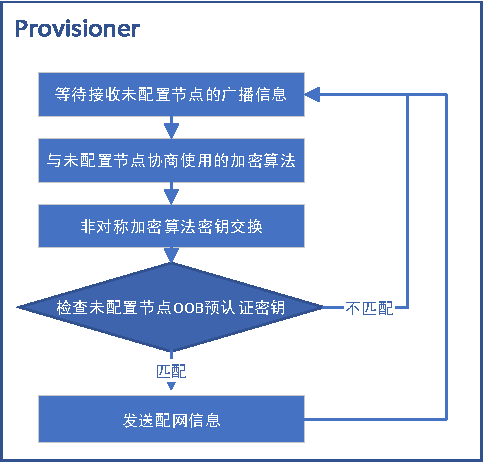
\includegraphics{flowchart_mesh_provisioner.pdf}
    \caption{基于BLE Mesh的智能家居平台BLE Mesh Provisioner节点流程图}
    \label{fig:flowchart_mesh_provisioner}
\end{figure}

\begin{figure}[H]
    \centering
    \begin{lstlisting}[language=C]
    static void startprovision(){
        static const char * uri_list[1];
        uri_list[0] = server_uri_index_select(m_nw_state.p_client_uri);
        //设置可用的配网器为自己
        prov_helper_provision_next_device(PROVISIONER_RETRY_COUNT, m_nw_state.next_device_address, uri_list, ARRAY_SIZE(uri_list));
        //开始对未配网列表中的首个设备进行配网
        prov_helper_scan_start();
        //配网完成,继续扫描未配网设备
    }

    static void start(){
        //程序入口
        ble_stack_init();
        mesh_init();
        //初始化蓝牙协议栈、Mesh协议栈
        nrf_mesh_enable();
        //启动Mesh协议栈
        while(true){
            startprovision();
            //进行配网操作
        }
    }
    \end{lstlisting}
    \caption{基于BLE Mesh的智能家居平台BLE Mesh Provisioner节点关键代码}
    \label{fig:code_mesh_provisioner}
\end{figure}

\subsection{网关端}
网关端在启动后扫描plugin/accessory和plugin/consumer目录下的插件,并一一加载设备层插件,获取所有节点列表后,再一一加载管理应用层插件,以协程的方式并行启动每个插件的工作函数,最后阻塞主协程。

\begin{figure}[H]
    \centering
    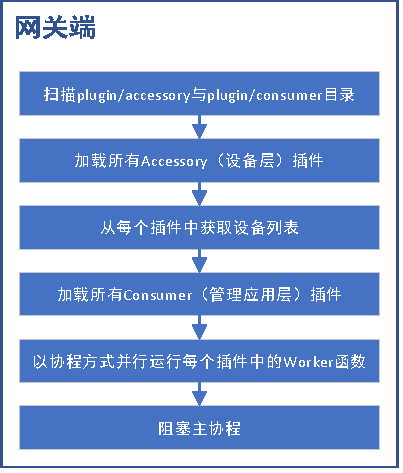
\includegraphics{flowchart_gateway.pdf}
    \caption{基于BLE Mesh的智能家居平台网关端流程图}
    \label{fig:flowchart_gateway}
\end{figure}

\begin{figure}[H]
    \centering
    \begin{lstlisting}[language=Go]
    func LoadAccessoryPlugin(){
        accpluginfiles,_:=ioutil.ReadDir(AccPluginDir)
        for _, f := range accpluginfiles{
            plug, err := plugin.Open(AccPluginDir+f.Name())
            sym, err := plug.Lookup("Plugin")
            accplugin := sym.(AccessoryPlugin)
            AccessoryPluginList = append(AccessoryPluginList, accplugin)
        }
    }
    func LoadConsumerPlugin(){
        conpluginfiles,_:=ioutil.ReadDir(ConPluginDir)
        for _, f := range conpluginfiles{
            plug, err := plugin.Open(ConPluginDir+f.Name())
            sym, err := plug.Lookup("Plugin")
            conplugin := sym.(ConsumerPlugin)
            ConsumerPluginList = append(ConsumerPluginList, conplugin)
        }
    }
    func InitAccessoryPlugin(){
        for _, accplugin := range AccessoryPluginList{
            accplugin.Init(Shutdown)
            AccessoryList = append(AccessoryList,accplugin.GetAccessoryList()...)
        }
    }
    func InitConsumerPlugin(){
	    for _, conplugin := range ConsumerPluginList{
	    	conplugin.Init(AccessoryList)
	    }
    }
    func main(){
        LoadAccessoryPlugin()
        LoadConsumerPlugin()
        InitAccessoryPlugin()
        InitConsumerPlugin()
        for _, accplugin := range AccessoryPluginList{
            go accplugin.Worker()
        }
        for _, conplugin := range ConsumerPluginList{
            go conplugin.Worker()
        }
        for{
            c := ""
            _, _ = fmt.Scanln(&c)
            if c == "stop"{Shutdown()}
        }
    }
    \end{lstlisting}
    \caption{基于BLE Mesh的智能家居平台网关端关键代码}
    \label{fig:code_gateway}
\end{figure}

\subsection{移动端}

\subsubsection{连接设备}
移动端在用户点击连接设备后,可选择通过蓝牙连接以及通过WLAN连接。

点击通过蓝牙连接,进入蓝牙扫描状态,搜索附近的蓝牙Mesh节点,弹出列表让用户选择后连接,即可通过单一节点代理入网,控制整个网络中的节点及所连接的模块。

点击通过WLAN连接,进入局域网扫描状态,搜索整个网络中已启用WebSocket插件的网关端,弹出列表让用户选择后连接,即可访问网关设备层中的所有节点及所连接的模块。

\begin{figure}[H]
    \centering
    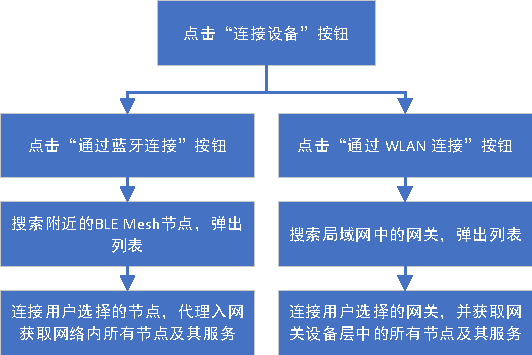
\includegraphics{flowchart_mobile_connect.pdf}
    \caption{基于BLE Mesh的智能家居平台移动端连接设备流程图}
    \label{fig:flowchart_mobile_connect}
\end{figure}

\begin{figure}[H]
    \centering
    \begin{lstlisting}[language=Java]
    BluetoothAdd() {
        meshnodes = scanMeshNodes();
        for(int i=0;i<meshnodes.length;i++){
          meshnodewidgets.add(Card(child: ListTile(onTap: (){
            connectmeshnode(meshnodes[i]);
          },leading: Icon(Icons.bluetooth),title: Text(meshnodes[i].name))));
        }
        showModalBottomSheet(context:this.context,builder:(BuildContext context) {
          return new ListView(children: <Widget>[
            Padding(padding:EdgeInsets.all(20),child:Text("选择 BLE Mesh 节点",textAlign: TextAlign.left,
              style: TextStyle(fontWeight: FontWeight.bold,fontSize: 20),)),
            ]+meshnodewidgets);
        });
    }
    \end{lstlisting}
    \caption{基于BLE Mesh的智能家居平台移动端通过蓝牙连接关键代码}
    \label{fig:code_mobile_connect_ble}
\end{figure}

\begin{figure}[H]
    \centering
    \begin{lstlisting}[language=Java]
    IPAdd() {
        ipnodes = scanIPNodes();
        for(int i=0;i<ipnodes.length;i++){
          ipnodewidgets.add(Card(child: ListTile(onTap: (){
            connectipnode(ipnodes[i]);
          },leading: Icon(Icons.router),title: Text(ipnodes[i].name),subtitle: Text(ipnodes[i].address))));
        }
        showModalBottomSheet(context:this.context,builder:(BuildContext context) {
          return new ListView(children: <Widget>[
            Padding(padding:EdgeInsets.all(20),child:Text("选择网关",textAlign: TextAlign.left,
              style: TextStyle(fontWeight: FontWeight.bold,fontSize: 20),)),
            ]+ipnodewidgets);
        });
    }
    \end{lstlisting}
    \caption{基于BLE Mesh的智能家居平台移动端通过WLAN连接关键代码}
    \label{fig:code_mobile_connect_wlan}
\end{figure}

\subsubsection{控制配件}
在配件列表中,点击可控制的服务后,进行电源状态的切换或弹出其他可调整项,之后将更新发送至连接的BLE Mesh节点或网关端,完成配件的控制。

\begin{figure}[H]
    \centering
    \begin{lstlisting}[language=Java]
    case SERVICE_LIGHTBULB:
        Characteristic c = srv.getCharacteristic(CHAR_ON);
        srv.name = "灯泡";
        value = dynamictoT<bool>(c.value)?"开":"关";
        icon = Icons.lightbulb_outline;
        onclick = (){
            c.value = !dynamictoT<bool>(c.value);
            if(srv.ble){
                bleupdate(srv.aid,c.cid);
            }else{
                wlanupdate(srv.aid,c.cid);
            }
        }
    \end{lstlisting}
    \caption{基于BLE Mesh的智能家居平台移动端控制灯泡服务关键代码}
    \label{fig:code_mobile_control_lightbulb}
\end{figure}

\subsubsection{自动化}
在自动化列表中,点击添加自动化按钮后,弹出选择触发服务菜单,选择用于触发的服务后,进入对应服务的条件界面,设置条件后点击下一步弹出选择操作服务菜单,进入对应服务的操作界面,设置操作后点击完成即添加完成。

\begin{figure}[H]
    \centering
    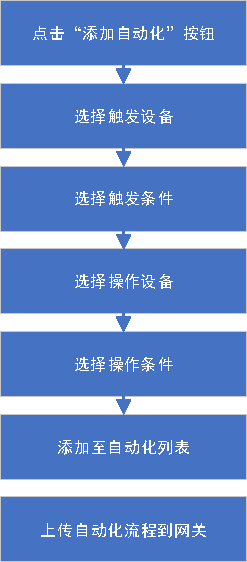
\includegraphics{flowchart_mobile_add_automation.pdf}
    \caption{基于BLE Mesh的智能家居平台移动端添加自动化流程图}
    \label{fig:flowchart_mobile_connect}
\end{figure}

\begin{figure}[H]
    \centering
    \begin{lstlisting}[language=Java]
    AddAutomation(){
        automation = new Automation();
        automation.trigger = gettriggerfrommodal();
        automation.when = getwhenfrommodal();
        automation.opservice = getopsrvfrommodal();
        automation.op = getopfrommodal();
        wlanaddautomation(automation);
        automationlist.add(automation);
    }
    \end{lstlisting}
    \caption{基于BLE Mesh的智能家居平台移动端添加自动化关键代码}
    \label{fig:code_mobile_add_automation}
\end{figure}